% ====== TAREA 2 MATEMATICAS APLICADAS ======
\documentclass{article}
\usepackage[utf8]{inputenc}
\usepackage[spanish]{babel}
\usepackage{amsmath, amsfonts, amssymb}
\usepackage{graphicx}
\usepackage[usenames]{color}
\usepackage[text={20cm,25cm},centering,top=1.5cm,bottom=1.5cm,letterpaper,showframe=false]{geometry}
\renewcommand{\baselinestretch}{1.5}
\parindent  = 0mm
\parskip    = 4mm
\definecolor{azul}{RGB}{10,80,190}
\definecolor{negro}{RGB}{0,0,0}
\definecolor{rojo}{RGB}{190,80,10}
\definecolor{verde}{RGB}{0,120,50}

\begin{document}
    \title{Tarea 2}
    \author{Careaga Carrillo Juan Manuel\\
            Quiróz Castañeda Edgar\\
            Soto Corderi Sandra del Mar}
    \date{Miércoles 10 de octubre de 2018}
    \maketitle
    \begin{enumerate}

        % Ejercicio 1
        \item {
            Encontrar la imagen de un triángulo con vértices $(0,0)$, $(1,1)$
            y $(0,1)$ bajo la transformación $x=u^2$ y $y=v$.

            \color{azul}
          Aplicamos la transformación a varios puntos del triángulo y obtenemos lo siguiente:
            \begin{center}
                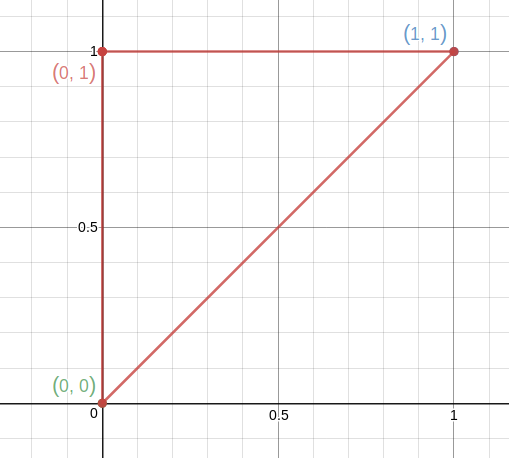
\includegraphics[width=6cm]{img/ejercicio1-1.png}
                \hspace{.5cm}
                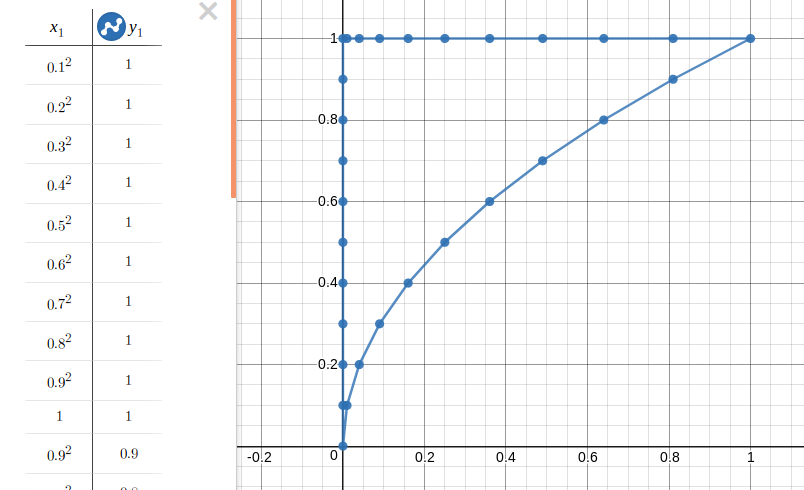
\includegraphics[width=9cm]{img/ejercicio1-2.png}
        	\end{center}
            En la imagen izquierda vemos el triángulo original, y en la derecha
            vemos la imagen del triángulo bajo la transformación.
            
            Podemos observar que la transformación convirtió el lado del triángulo que iba de $(0,0)$ a $(1,1)$ en una curva, ya que $x=u^2$, el resto de los lados parecen verse no afectados, pero los puntos tomados si cambiaron en posición, recorriéndose, ya que al tomar número decimales al cuadrado obtenemos coordenadas menores a las originales.
	    }

        % Ejercicio 2
        \pagebreak
        \item {
            Calcular
            \[
                \iint_{D}{e^{\frac{x-2y}{3x-y}}\,dA}
            \]
            con $D$ el paralelogramo acotado por las rectas $x-2y=0$, $x-2y=$,
            $3x-y=1$ y $3x-y=8$

            \color{azul}
            El paralelogramo $D$ lo podemos ver como la siguiente imagen:
            \begin{center}
                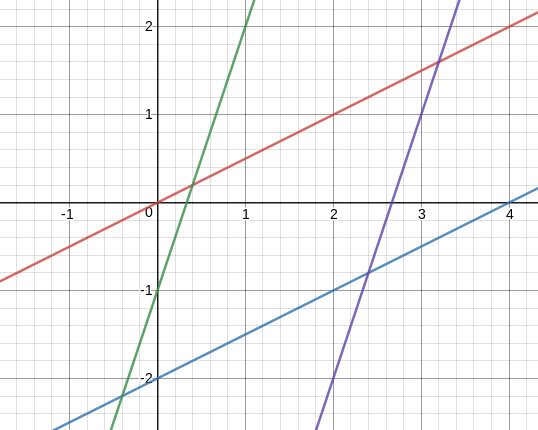
\includegraphics[width=6cm]{img/ejercicio2.png}
         	\end{center}
             Para facilitar la integral, realizaremos un cambio de variable
             y una transformación lineal con $D$.

             Obtenemos el Jacobiano de la siguiente forma:
             \[
                 \begin{bmatrix}
                     \frac{\partial x}{\partial u}&
                     \frac{\partial x}{\partial v}\\
                     \frac{\partial y}{\partial u}&
                     \frac{\partial y}{\partial v}\\
                 \end{bmatrix}
                 =
                 \begin{bmatrix}
                     -\frac{1}{5}
                     &\frac{2}{5}\\
                     -\frac{3}{5}
                     &\frac{1}{5}\\
                 \end{bmatrix}
                 =\frac{1}{5}
             \]
             Para la transformación, tomamos $u = x-2y$ y $v= 3x-y$.
            
             Despejando con un sistema de ecuaciones de $u$ y $v$, tenemos que
             $x = -(\frac{u-2v}{5})$ y  $y = -(\frac{3u-v}{5})$

             De ahí, si aplicamos la transformación en los lados del
             paralelogramo tenemos:
             $$T(x-2y=0) \Rightarrow (\frac{-u+2v}{5}) + 2(\frac{3u-v}{5}) =
             \frac{-u+2v+6u-2v}{5} = \frac{5u}{5} \Rightarrow u = 0$$
             $$T(x-2y=4) \Rightarrow (\frac{-u+2v}{5}) + 2(\frac{3u-v}{5}) =
             \frac{-u+2v+6u-2v}{5} = \frac{5u}{5} \Rightarrow u = 4$$
             $$T(3x-y=1) \Rightarrow -3(\frac{u-2v}{5}) + (\frac{3u-v}{5}) =
             \frac{-3u+6v+3u-v}{5} = \frac{5v}{5} \Rightarrow v = 1$$
             $$T(3x-y=8) \Rightarrow -3(\frac{u-2v}{5}) + (\frac{3u-v}{5}) =
             \frac{-3u+6v+3u-v}{5} = \frac{5v}{5} \Rightarrow v = 8$$

             La imagen del paralelogramo bajo la transformación es como la
             siguiente imagen, vemos que es un cuadrado, así que los límites
             de $u$ y $v$ son sencillos.
             \begin{center}
                 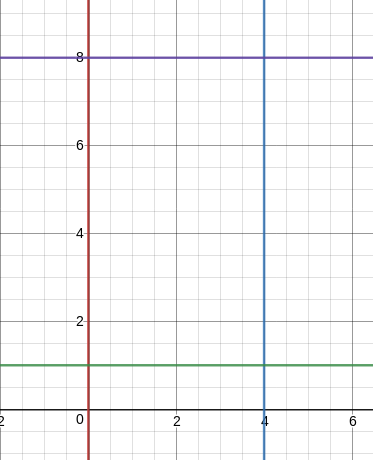
\includegraphics[width=5cm]{img/ejercicio2-1.png}
         	\end{center}
             De ahí, podemos resolver a nuestra integral doble como:
             \[
                \int_{1}^{8}{
                    \int_{0}^{4}{
                        \frac{1}{5} e^{\frac{u}{v}}
                    \,du}
                \,dv}
            \]
             Usando integración por sustitución tomando $s =\frac{u}{v}$,
             resolvemos directamente $du$
             \[
                = \frac{1}{5} \int_{1}^{8}{
                    v\left(e^{\frac{4}{v}} -1\right)
                \,dv}
            \]
            \[
                \int_{1}^{8}{
                    v\left(e^{\frac{4}{v}} -1\right)
                \,dv}
                =
                \int_{1}^{8}{
                    ve^{\frac{4}{v}}
                \,dv}
                -
                \int_{1}^{8}{v\,dv}
            \]
            \[
                \int_{1}^{8}{v\,dv}
                = \frac{v^2}{2}\Big|_1^8
                = \frac{63}{2}
            \]
             Usando integración por sustitución tomando $t =\frac{4}{v}$,
             $dt = -\frac{v^2}{4}dv$ y $v= \frac{4}{t}$
             \[
                \int_{1}^{8}{ve^{\frac{4}{v}}\,dv}
                = -16\int_{1}^{8}{\frac{e^{t}}{t^3}\,dt}
            \]
            Usando integración por partes donde $u = e^t$ y
            $dv = \frac{1}{t^3}$
            \[
                \int_{1}^{8}{\frac{e^{t}}{t^3}\,dt}
                = -\frac{e^t}{2t^2} + \int{-\frac{e^t}{2t^2}\,dt}
            \]
            Nuevamente por integración por partes donde $u = e^t$ y
            $dv = \frac{1}{2t^2}$
            \[
                \int{-\frac{e^t}{2t^2}\,dt}
                = -\frac{1}{2} \left(
                    -\frac{e^t}{t} + \int{\frac{e^t}{t}\,dt}
                \right)
            \]
            Finalmente, con la definición $Ei(t) = \int\frac{e^t}{t}dt$,
            resolvemos el resto de integral. También regresamos a los valores
            originales
            \[
                \int_{1}^{8}{ve^{\frac{4}{v}}\,dv}
                = \left[
                    -16\left(
                        -\frac{1}{32}e^{\frac{4}{v}}v^2
                        +\frac{1}{2}\left(-\frac{1}{4}\right)e^{\frac{4}{v}}v
                        +Ei\left(\frac{4}{v}\right)
                    \right)
                \right]_1^8
            \]
            De todo lo anterior, el resultado sería:
            \[
                \int_{1}^{8}{
                    \int_{0}^{4}{
                        -\frac{7}{25}e^{\frac{u}{v}}
                    \,du}
                \,dv}
                =\left(\frac{1}{5}\right)\left(48\sqrt{e}
                -8Ei\left(\frac{1}{2}\right)
                -32
                -\frac{5e^4 - 16Ei(4)}{2}\right)
            \]
        }

        % Ejercicio 3
        \item {
            Hallar el volumen del elipsoide
            \[
                \frac{x^2}{a^2}+\frac{y^2}{b^2}+\frac{z^2}{c^2}\leq 1
            \]

            \color{azul}
            Hallar el volumen de forma típica nos daría una integral triple
            bastante compleja, así que para auxiliarnos, transformamos la
            elipsoide a coordenas esféricas y realizamos un cambio de variables.
            \begin{center}
                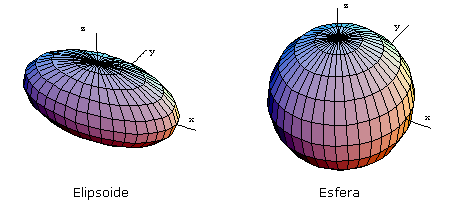
\includegraphics[width=10cm]{img/elipsoide.png}
        	\end{center}
            Tomamos la siguiente transformación, basada en coordenadas esféricas:
            \begin{align*}
                x &= ar\sen\gamma\cos{\theta}\\
                y &= br\sen\gamma\sen{\theta}\\
                z &= cr\cos\gamma
            \end{align*}

            El jacobiano sería la multiplicación de $abc$ con el jacobiano de
            coordenadas esféricas que vimos en clase es $r^2\sen{\gamma}$. De
            ahí, el jacobiano es $abcr^2\sen{\gamma}$

            El elipsoide es simétrico respecto al origen, los ejes y los planos
            de coordenadas. Además las secciones con planos paralelos a los
            coordenados son elipses (caso particular: circunferencia). De esta
            forma si vemos al elipsoide en coordenas esféricas podemos
            representar su volumen de esta manera:
        	\[
                \int_{0}^{1}{
                    \int_{0}^{2\pi}{
                        \int_{0}^{\pi}{
                            abcr^2\sen\gamma
                        \,d\gamma}
                    \,d\theta}
                \,dr}
            \]
            Debido a que las variables son independientes una de otra podemos
            resolver la integral así:
            \[
                (abc)
                \left(\int_{0}^{1}r^2 dr\right)
                \left(\int_{0}^{2\pi} d\theta\right)
                \left(\int_{0}^{\pi}\sen{\gamma} d\gamma\right)
                =
                (abc)
                \left(\frac{r^3}{3}\Big|_0^1\right)
                \left(\theta\Big|_0^{2\pi}\right)
                \left(-\cos{\gamma}\Big|_0^{\pi}\right)
                =
                (abc)\left(\frac{1}{3}\right)
                \left(2\pi\right)(2)
                =
                \frac{4}{3}\pi abc
            \]
            Por lo tanto, el volumen del elipsoide es
            $\displaystyle \frac{4}{3}\pi abc$.
        }

        % Ejercicio 4
        \item {
            Hallar el área acotada por la lemniscata
            \(
                \left(x^2+y^2\right)^2=2a^2\left(x^2-y^2\right)
            \).

            \color{azul}
          	Para pasar de coordenadas rectangulares a polares, se tiene que
            $r^2 = x^2+y^2$, $x = r\cos \theta$ y  $y = r\sen \theta$.
            Entonces, la ecuación de la lemniscata se puede reescribir como
            \begin{align*}
                (r^2)^2 &= 2a^2(r^2 \cos^2 \theta - r^2 \sen^2 \theta)\\
                (r^2)^2 &= 2a^2r^2(\cos^2 \theta - \sen^2 \theta)\\
                (r^2)^2 &= 2a^2r^2\cos2\theta\\
                r^2 &= 2a^2\cos2\theta\\
                r &= a\sqrt{2\cos2\theta}
            \end{align*}
            Para calcular el área baja un curva polar en un rango
            $\theta \in[\alpha, \beta]$, se tiene que definir una
            suma de Riemann. En lugar de utilizar rectángulos de altura $f(x*)$
            ,base $\Delta x$ y área $f(x*)\Delta x$ en un rango $x\in[a, b]$,
            se tienen que usar fragmentos de círculo de radio $r(\theta *)$
            y de ángulo $\Delta \theta$.\\
            El área de un fragmento de círculo de radio $r$ y ángulo $\theta$
            es el área total del círculo $\pi r^2$ por la fracción del círculo
            que representa el ángulo $\frac{\theta}{2\pi}$. Por lo que es área
            sería $\frac{\pi r ^2\theta}{2\pi} = \frac{r^2\theta}{2}$.\\
            Entonce la suma de Riemann sería

            \[\sum_{i = 1}^n {\frac{r(\theta *)^2}{2}}\Delta \theta\]

            Y el área bajo la curva polar sería

            \[
                \lim_{n \to \infty}\sum_{i = 1}^n {\frac{r(\theta *)}{2}}\Delta \theta
                = \frac{1}{2}\int_\beta^\alpha {r(\theta)^2}d\theta
            \]

            Volviendo a la lemniscata, notemos que es simétrica respecto al eje
            $x$ y al eje $y$, por lo que se puede considerar sólo el primer
            cuandrante y multiplicar lo obtenido por 4 para tener el área total.\\
            Además, la función que se tiene del radio $r = a\sqrt{2\cos2\theta}$
            no está definida para valores negativos de $\cos2\theta$.
            \[
                \cos2\theta \geq 0 \implies 0 \leq 2\theta \leq \frac{\pi}{2}
                \implies 0 \leq \theta \leq \frac{\pi}{4}
            \]
            Entonces los límites de integración son 0 y $\frac{\pi}{4}$.\\
            El área de un cuarto de la lemniscata es

            \begin{align*}
                \frac{1}{2}\int_0^{\frac{\pi}{4}}{r(\theta)^2 d\theta}
                &= \frac{1}{2}\int_0^{\frac{\pi}{4}}{(a\sqrt{2\cos2\theta})^2 d\theta}
                = \frac{1}{2}\int_0^{\frac{\pi}{4}}{a^2 2\cos2\theta d\theta}
                = \frac{1}{2}\cdot 2a^2 \int_0^{\frac{\pi}{4}}{\cos2\theta d\theta}\\
                &= a^2 \Big (\frac{\sen 2\theta}{2} \Big |_0^{\frac{\pi}{4}} \Big )
                = \frac{a^2}{2} (\sen (2\cdot\frac{\pi}{4}) - \sen (2\cdot0))
                = \frac{a^2}{2} (1-0) = \frac{a^2}{2}
            \end{align*}
            Por lo que el área total de la lemniscata es
            $4 \cdot \frac{a^2}{2} = 2a^2$
        }

        % Ejercicio 5
        \item {
            Evaluar la integral iterada
            \[
                \int_{0}^{2}{
                    \int_{-\sqrt{2x-x^2}}^{\sqrt{2x-x^2}}{
                        \int_{0}^{x^2+y^2}{
                            \sqrt{x^2+y^2}
                        \,dz}
                    \,dy}
                \,dx}
            \]
            y bosquejar la región de integración $W$.

            \color{azul}
            Pasando a coordenadas cilíndricas.\\
            Se tiene que $r^2 = x^2 + y^2$, $x = r\cos(\theta)$, $y = r\sen(\theta)$
            y $z = z$.\\
            La función $\sqrt{x^2+y^2}$ se vuelve $r \cdot r = r^2$, por el jacobiano.\\
            Los límites de $z$ se vuelven 0 y $r^2$.

            Para los límites de $r$ y de $\theta$ notemos que
            \begin{align*}
                &-\sqrt{2x-x^2} \leq y \leq \sqrt{2x-x^2}
                \implies y^2 \leq 2x-x^2 \implies y^2 + x^2 - 2x \leq 0\\
                &\implies y^2 + x^2 - 2x + 1 \leq 1
                \implies (y - 0)^2 + (x - 1)^2 \leq 1^2
            \end{align*}
            Por lo que los límites de $y$ son un círculo de radio $1$ centrado
            en $(1, 0)$.\\
            Y como los límites en $x$ son precisamente 0 y 2, entonces el área
            de integración definida por lo límites de $x$ y $y$ son todos los
            puntos dentro de ese círculo.\\
            Hay que reescribir ese círculo como función polar.
            \begin{align*}
                (y-0)^2+(x-1)^2=1^2
                &\implies y^2+x^2-2x+1 = 1\\
                &\implies y^2+x^2 = 2x\\
                &\implies r^2 = 2r\cos(\theta)\\
                &\implies r = 2\cos(\theta)
            \end{align*}
            Entonces los límites del radio son 0 y $2\cos(\theta)$.\\
            Faltan los rangos de $\theta$. Como el radio es una distancia,
            siempre es positivo. Entonces
            \[
                \cos(\theta) \geq 0 \implies 0 \leq \theta \leq \frac{\pi}{2},
                \frac{3\pi}{2} \leq \theta \leq 2 \pi
            \]
            O más simplemente $-\frac{\pi}{2} \leq \theta \leq \frac{\pi}{2}$.\\
            Entonces, la integral cilíndrica es
            \[
                \int_{-\frac{\pi}{2}}^{\frac{\pi}{2}}{
                    \int_{0}^{2\cos(\theta)}{
                        \int_{0}^{r^2}{
                            r^2
                        \,dz}
                    \,dr}
                \,d\theta}
            \]

            Primero
            \[
                \int_{0}^{r^2}{r^2dz} = (r^2 \cdot z) \Big |_0^{r^2}
                = r^2 (r^2 - 0) = r^4
            \]
            Luego
            \[
                \int_{0}^{2\cos(\theta)}{r^4dr}
                = \frac{r^5}{5} \Big |_{0}^{2\cos(\theta)}
                = \frac{1}{5} ((2\cos(\theta))^5 - 0^5)
                = \frac{32\cos^5(\theta)}{5}
            \]
            Finalmente
            \begin{align*}
                &\int_{-\frac{\pi}{2}}^{\frac{\pi}{2}}{\frac{32\cos^5(\theta)}{5}d\theta}
                = \frac{32}{5} \int{\cos^5(\theta)d\theta}
                = \frac{32}{5} \int{(\cos^2(\theta))^2\cos(\theta)d\theta}\\
                &= \frac{32}{5} \int{(1-\sen^2(\theta))^2\cos(\theta)d\theta}
                = \frac{32}{5} \int{(1-u^2)^2du}
                = \frac{32}{5} \int{(1-2u^2+u^4)du}\\
                &= \frac{32}{5} (u - \frac{2u^3}{3} + \frac{u^5}{5})
                = \frac{32}{5} (\sen(\theta) - \frac{2\sen(\theta)^3}{3}
                + \frac{\sen(\theta)^5}{5}) \Big |_{-\frac{\pi}{2}}^{\frac{\pi}{2}}\\
                &= \frac{32}{5} ((1-\frac{2}{3}+\frac{1}{5})-(-1+\frac{2}{3}-\frac{1}{5}))
                = \frac{32}{5} \cdot 2(1-\frac{2}{3}+\frac{1}{5})\\
                &= \frac{32}{5} \cdot \frac{8}{15} = \frac{256}{75}
            \end{align*}
	    }

        % Ejercicio 6
        \item {
            Calcular la masa del sólido que se encuentra fuera de la esfera
            $x^2+y^2+^z2=1$ y dentro de la esfera $x^2+y^2+z^2=2$ suponiendo
            que la densidad en un punto $P$ es directamente proporcional al
            cuadrado de la distancia de $P$ al centro de la esfera.

            \color{azul}
            % Respuesta
        }

        % Ejercicio 7
        \item {
            Determinar los números reales $\lambda$ para los que
            \[
                \iint_D {\frac{dA}{\left(x^2+y^2\right)^\lambda}}
            \]
            es convergente, con $D$ el disco unitario con centro en el origen.

            \color{azul}
            % Respuesta
            \begin{center}
                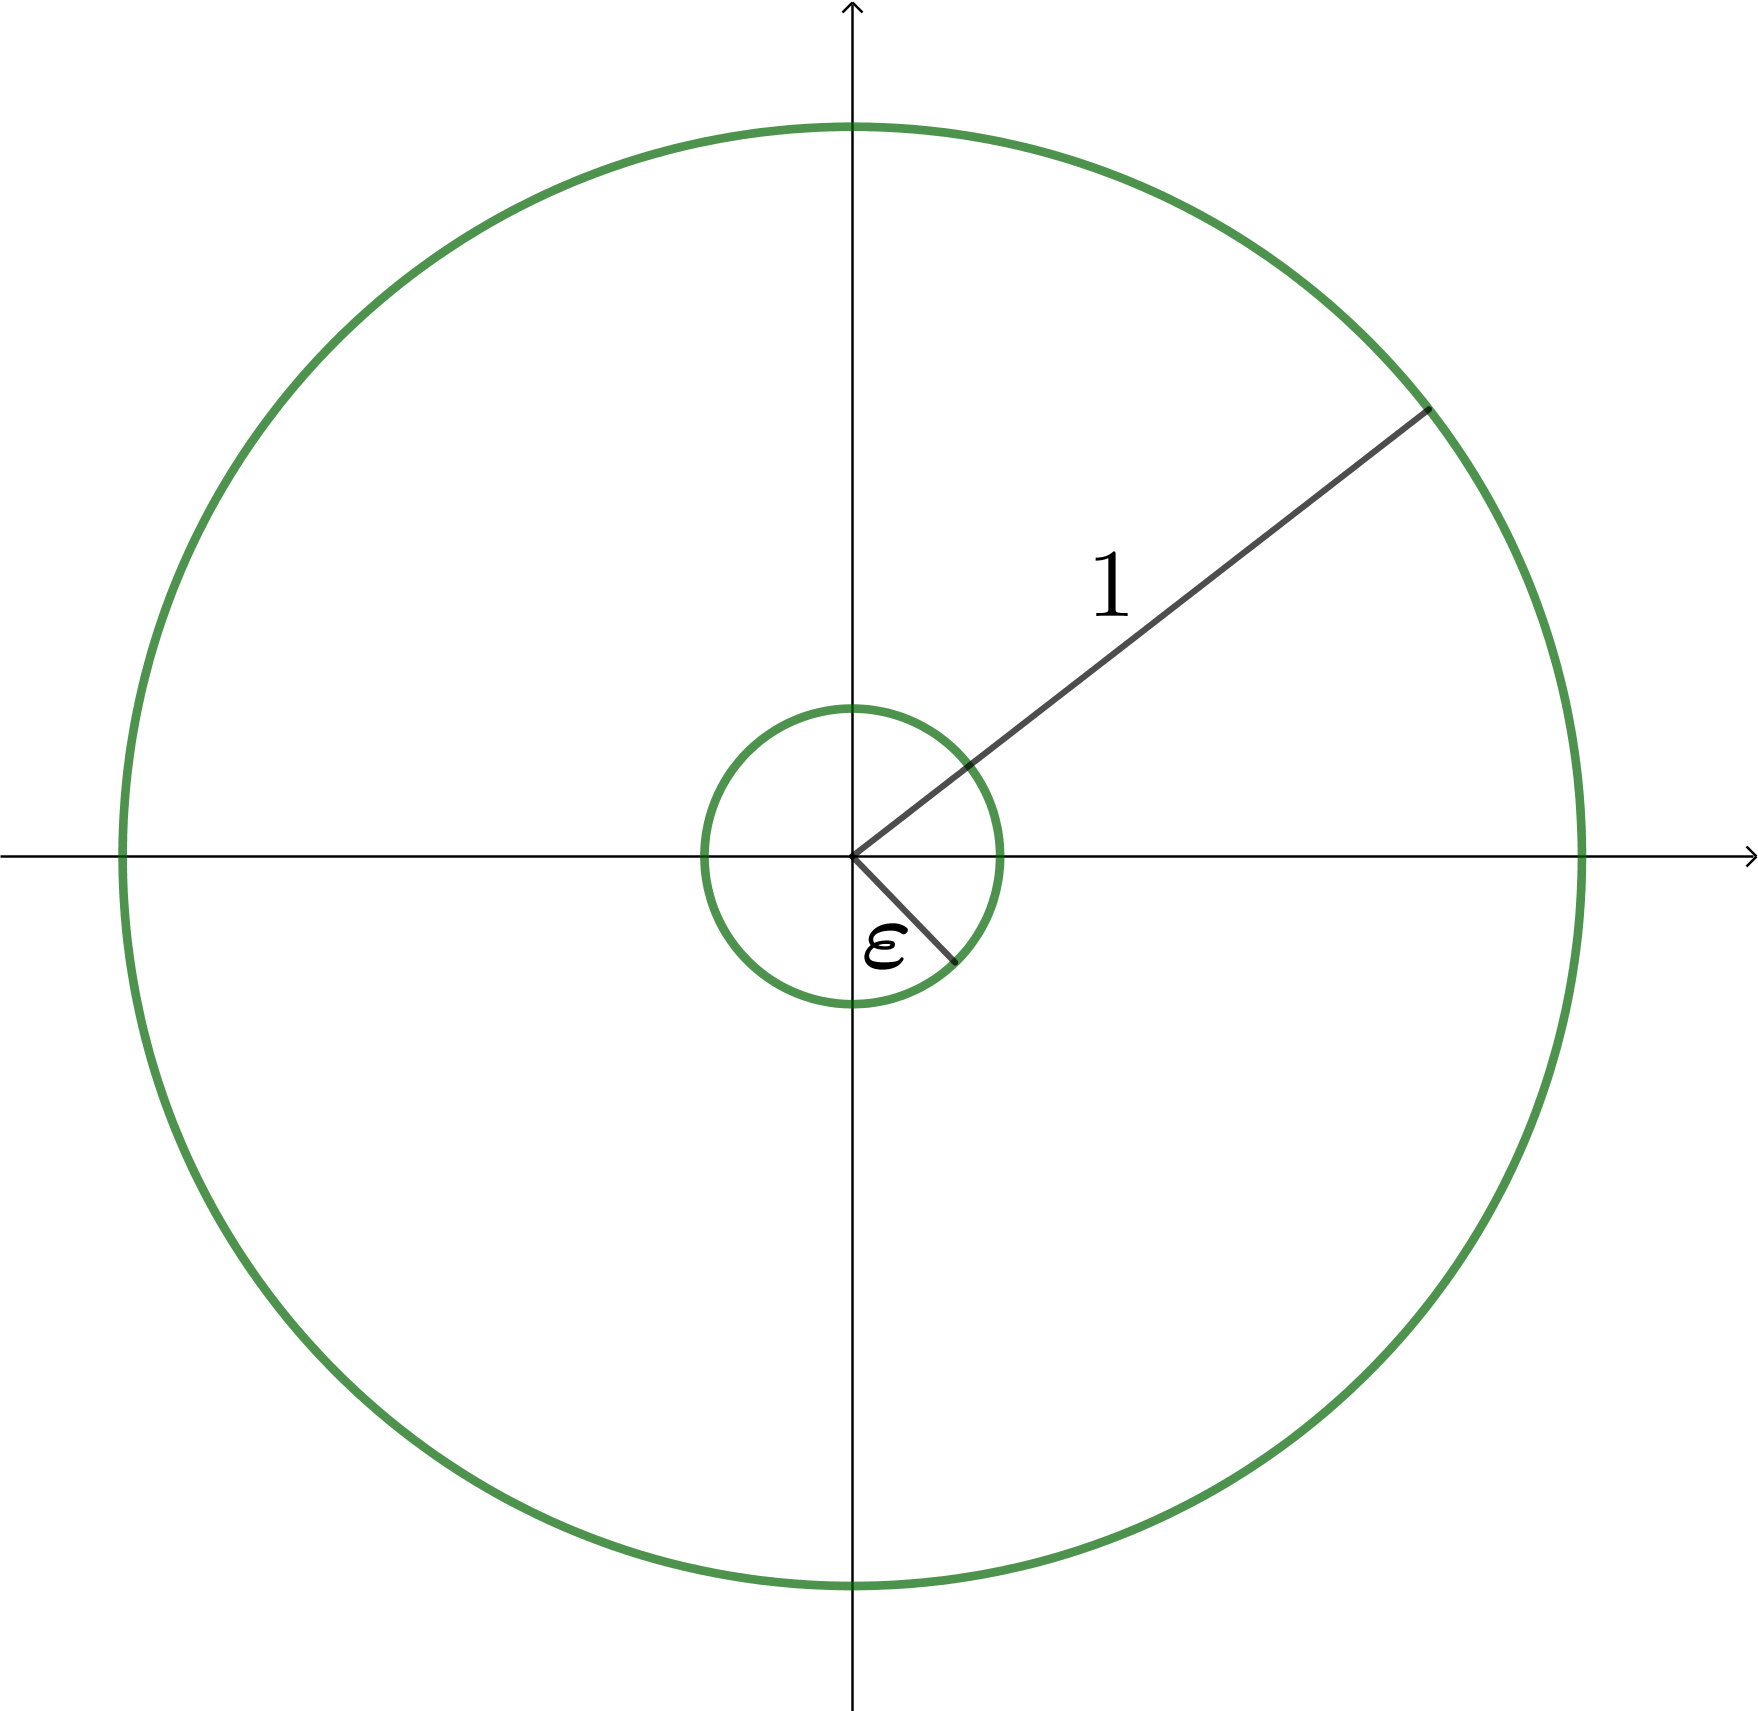
\includegraphics[width=4cm]{img/ej7.png}
            \end{center}
            La función $\displaystyle f(x)=\frac{1}{(x^2+y^2)^\lambda}$ no está
            definida cuando $x^2+y^2=0$, así que definimos una nueva región de
            integración $D_\varepsilon = \left\{(x,y)\in\mathbb{R}^2 |
            \varepsilon\leq x^2+y^2\leq 1\right\}$ y hacemos $\varepsilon
            \to 0$
            \[
                \iint_D {\frac{dA}{\left(x^2+y^2\right)^\lambda}}
                =\lim_{\varepsilon\to 0}{
                    \iint_{D_\varepsilon}{
                        \frac{dA}{\left(x^2+y^2\right)^\lambda}
                    }
                }
            \]
            para resolver la integral, conviene hacer una transformación a
            coordenadas polares
            \[
                \iint_D {\frac{dA}{\left(x^2+y^2\right)^\lambda}}
                =\int_{0}^{2\pi}{
                    \int_{0}^{1}{
                        \frac{r}{r^{2\lambda}}
                    \,dr}
                \,d\theta}
                =\lim_{\varepsilon\to 0}{
                    \int_{0}^{2\pi}{
                        \int_{\varepsilon}^{1}{
                            r^{1-2\lambda}
                        \,dr}
                    \,d\theta}
                }
            \]
            resolviendo la integral iterada (considerando $\lambda \ne 1$)
            \begin{align*}
                \lim_{\varepsilon\to 0}{
                    \int_{0}^{2\pi}{
                        \int_{\varepsilon}^{1}{
                            r^{1-2\lambda}
                        \,dr}
                    \,d\theta}
                }
                &=\lim_{\varepsilon\to 0}{
                    \int_{0}^{2\pi}{
                        \left[
                            \frac{r^{2-2\lambda}}
                                 {2-2\lambda}
                        \right]_{\varepsilon}^{1}
                    \,d\theta}
                }\\[.2cm]
                &=\lim_{\varepsilon\to 0}{
                    \int_{0}^{2\pi}{
                        \frac{1-\varepsilon^{2(1-\lambda)}}
                             {2(1-\lambda)}
                    \,d\theta}
                }\\[.2cm]
                &=\lim_{\varepsilon\to 0}{
                    \frac{2\pi[1-\varepsilon^{2(1-\lambda)}]}
                         {2(1-\lambda)}
                }\\[.2cm]
                &=\lim_{\varepsilon\to 0}{
                    \frac{\pi[1-\varepsilon^{2(1-\lambda)}]}
                         {1-\lambda}
                }
            \end{align*}
            Haciendo un análisis de ésta última expresión, concluimos que:
            \begin{itemize}
                \item si $\lambda>1$, entonces $1-\lambda>0$ y
                    $\varepsilon^{2(1-\lambda)}\to\infty$ (diverge)
                \item es cuando $\lambda<1$, entonces la integral converge.
            \end{itemize}

        }

        % Ejercicio 8
        \item {
            Calcular
            \[
                \iint_D {xye^{-\left(x^2+y^2\right)}\,dA}
            \]
            con $x\geq 0$ y $0\leq y\leq 1$.

            \color{azul}
            % Respuesta
            Notemos que la región de integración es infinita, como se ve en la
            siguiente figura
            \begin{center}
                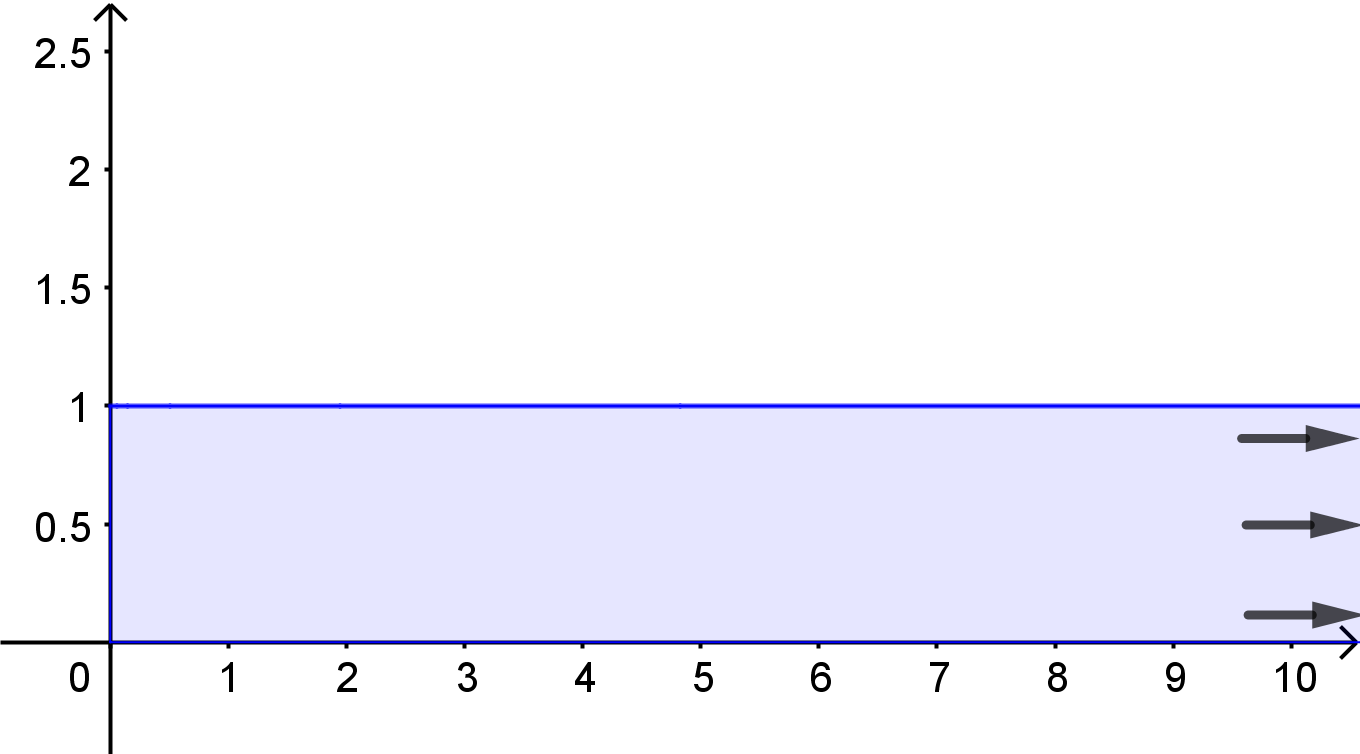
\includegraphics[width=5cm]{img/ej8.png}
            \end{center}
            Así que la integral iterada a resolver es
            \[
                \int_{0}^{\infty}{
                    \int_{0}^{1}{
                        xye^{-(x^2+y^2)}
                    \,dy}
                \,dx}
            \]
            Sustituimos ese infinito con una nueva variable $t$ y hacemos que
            ésta tienda hacia infinito
            \begin{align*}
                \lim_{t\to\infty}{
                    \int_{0}^{t}{
                        \int_{0}^{1}{
                            xye^{-(x^2+y^2)}
                        \,dy}
                    \,dx}
                }
                &=\lim_{t\to\infty}{
                    \int_{0}^{t}{
                        x\left[-\frac{1}{2}e^{-(x^2-y^2)}\right]_0^1
                    \,dx}
                }\\[.3cm]
                &=-\frac{1}{2}\lim_{t\to\infty}{
                    \int_{0}^{t}{
                        x\left[e^{-(x^2+1)}-e^{-x^2}\right]
                    \,dx}
                }\\[.3cm]
                &=-\frac{1}{2}\lim_{t\to\infty}{
                    \int_{0}^{t}{
                        xe^{-x^2}\left[e^{-1}-1\right]
                    \,dx}
                }\\[.3cm]
                &=-\frac{e^{-1}-1}{2}\lim_{t\to\infty}{
                    -\frac{1}{2}\left[-\frac{1}{2}e^{-x^2}\right]_{0}^{t}
                }\\[.3cm]
                &=\frac{e^{-1}-1}{4}\lim_{t\to\infty}{
                    \left(e^{-t^2}-1\right)
                }
            \end{align*}
            Simplificamos la expresión $\frac{e^{-1}-1}{4}=\frac{1-e}{4e}$ y al
            calcular el límite $e^{-t^2}\to 0$ por lo que el límite es
            $-1$ y el resultado de la integral es $\displaystyle\frac{e-1}{4e}$
        }
    \end{enumerate}
\end{document}
